%% LaTeX template file for Doctor Thesis
%% 
%% This template has Japanese characters,
%% so you have to compile this by pLaTeX.
\RequirePackage{plautopatch}
\documentclass[12pt,dvipdfmx]{report}
\usepackage{icsdoctor} % Style file for ICS
\usepackage{graphicx} % For figure
\usepackage{tabularx} % for table.
\usepackage{latexsym} % for mathematical operators
\usepackage{verbatim}
\usepackage{moreverb}
%\usepackage{makeidx} % for index
\usepackage{url} % for describing url
%\makeindex

\newtheorem{definition}{Definition}[chapter]
\newtheorem{algorithm}{Algorithm}[chapter]

\begin{document}

\etitle{English Title}
\jtitle{Japanese Title}
\author{Your Name}
\affiliation{Graduate School of Science and Engineering,\\Saitama University}
\supervisor{Supervisor's Name}
\date{December 20XX}
\maketitle

\pagenumbering{roman} % Don't delete that.
\begin{abstract}
\addcontentsline{toc}{chapter}{Abstract} % Don't delete that.
%\setlength{\baselineskip}{1.6\baselineskip}

abstract
 
\end{abstract}

\chapter*{Acknowledgments}
\addcontentsline{toc}{chapter}{Acknowledgments} % Don't delete that.
\setcounter{page}{3} % Please fix the page number.

{%
\hspace{1em} Special thanks are due to my thesis supervisor Professor
XXXX for his invaluable support and guidance through the hard
moments of graduate school.
I am also grateful to my dissertation committee: Professor XXXXX for
their support, valuable feedback, and insightful ideas to this research.
}%

% Don't delete following sentences.
\tableofcontents
\listoffigures
\addcontentsline{toc}{chapter}{List of figures}
\listoftables
\addcontentsline{toc}{chapter}{List of tables}


%\setlength{\baselineskip}{1.6\baselineskip}

\chapter{Introduction}
\pagenumbering{arabic} % Don't delete that.
\setcounter{page}{1}   % Don't delete that.

\section{Background and Motivation}
\section{Earlier research}
\section{Structure of this thesis}
The rest of thesis organised as follows:
Chapter \ref{chap:second} explains ... 
Chapter \ref{chap:third} gives conclusion and future works.

\chapter{Hogehoge} \label{chap:second}

hahahahah.

\chapter{Fugafuga}
\section{Foofoo}
hehehehe

\section{Hyohyo}

fufufufufufufu.

\chapter{HooHoo} \label{chap:third}

\section{Example of figures}

Figure \ref{fig:reasoning_engine} shows ...


 \begin{figure}[tb]
 \begin{center}
   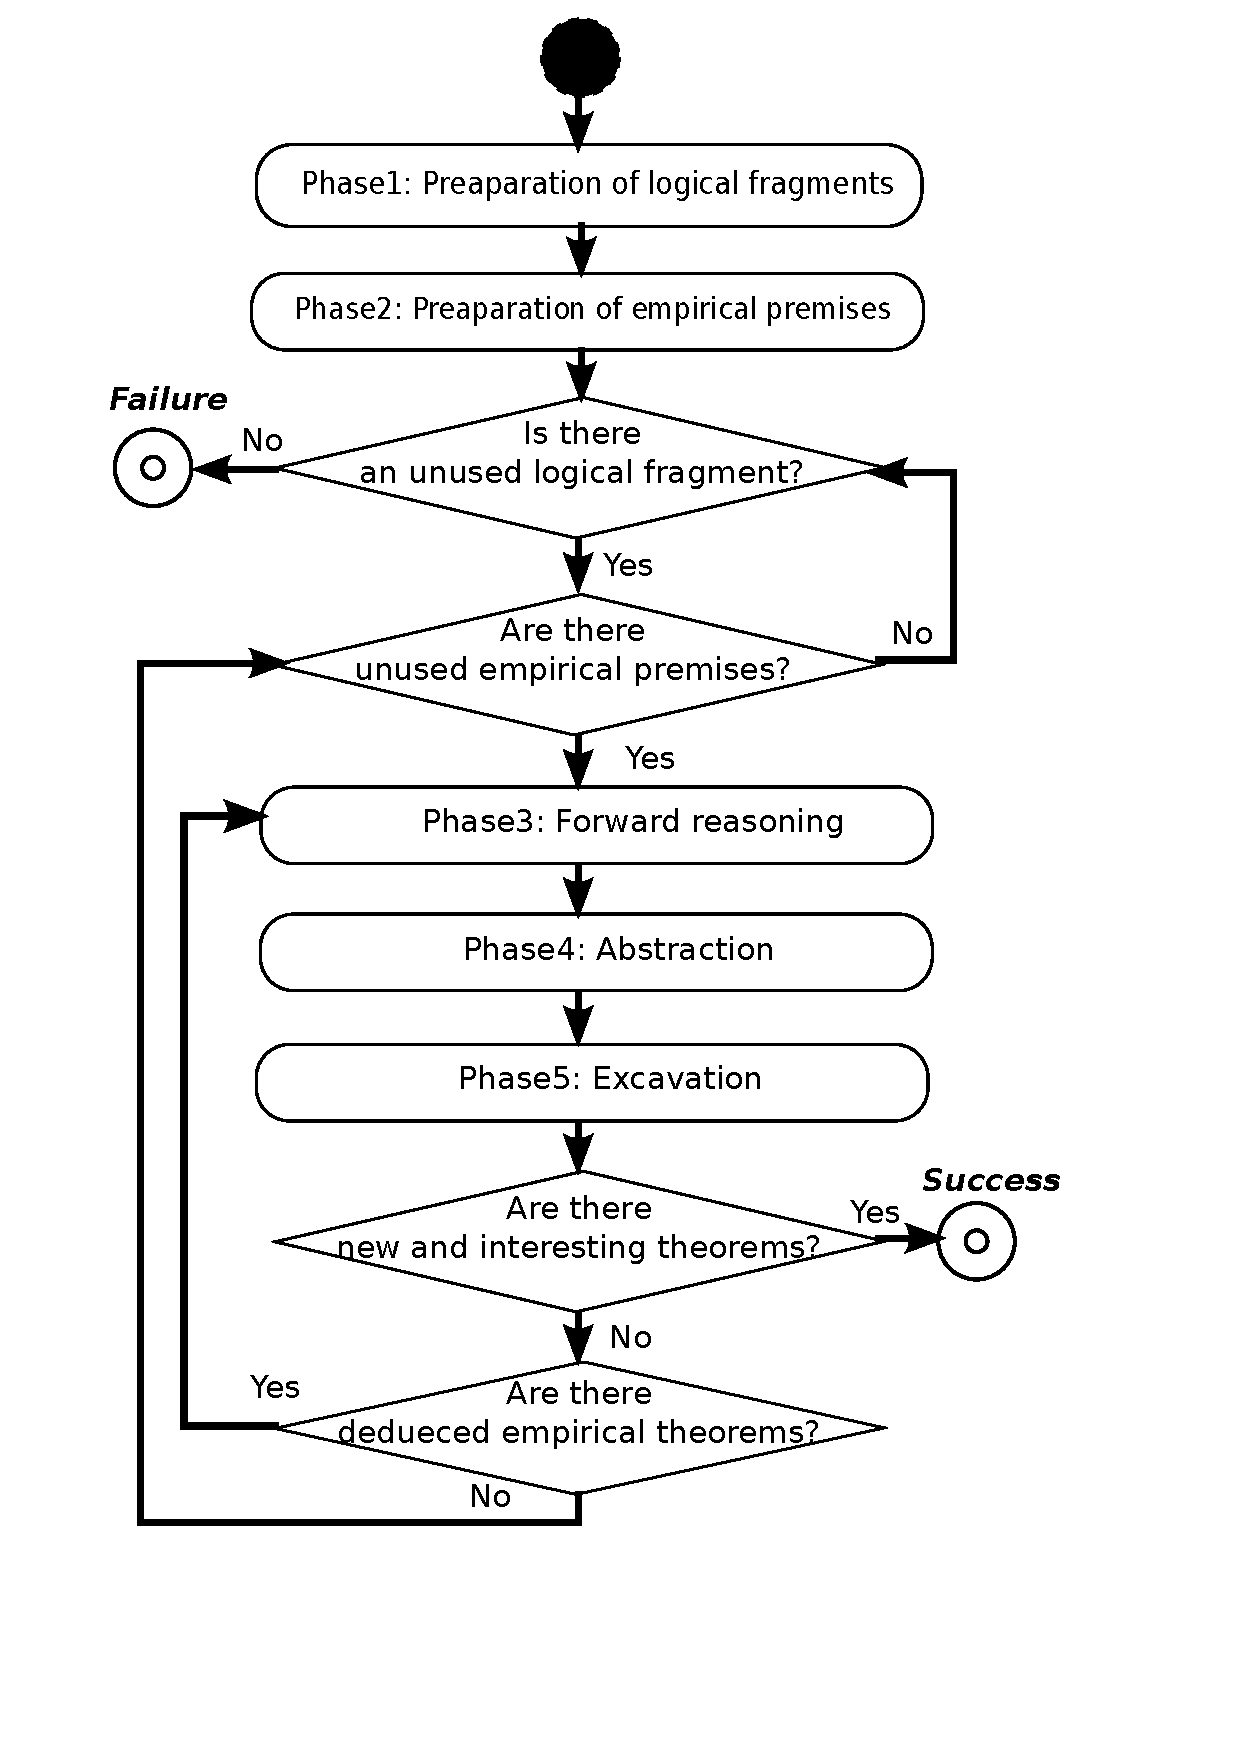
\includegraphics[scale=0.6]{fig/reasoning_engine.pdf}
  \caption{The relationship among the parts of EnCal}
  \label{fig:reasoning_engine}
 \end{center}
\end{figure}

 \section{Example of tables}

 Table \ref{tab:num_of_schemata_satisfied_srp} shows ...
 
 \begin{table}[tb]
\begin{center}
\caption{The number of elements of $F_{k}(CML)$ and $FS_{k}(CML)$}
\label{tab:num_of_schemata_satisfied_srp}
 \begin{tabular}{c l l}
  \hline
 degree & $F_{k}(CML)$ &$FS_{k}(CML)$ \\
    & (a)&  (b)\\ 
  \hline
  \hline
  1 &  $1.60 \times 10^{1}$ & $4.00 \times 10^{0}$\\
  2 & $2.26 \times 10^{3}$ & $2.60 \times 10^{2}$  \\
  3 & $1.67 \times 10^{8}$ & $8.90 \times 10^{6}$\\
  4 & $2.92 \times 10^{19}$ & $5.15 \times 10^{17}$\\
  5 & $1.63 \times 10^{45}$ & $6.31 \times 10^{42}$\\
  6 & $4.29 \times 10^{103}$ & $2.13 \times 10^{100}$\\
  7 & $1.02 \times 10^{235}$ & $3.09 \times 10^{230}$\\
  8 & $8.15 \times 10^{527}$ & $5.61 \times 10^{521}$\\ 
  \hline
 \end{tabular}
\end{center}
\end{table}


\chapter{Conclusion}
\section{Summary}

We have ...

\section{Future Works}

Future works are as follows: ...


\chapter*{Publications}
\addcontentsline{toc}{chapter}{Publications}

\begin{list}%
 {} %default label
 {} %formatting parameter
 \item Refereed papers
       \begin{itemize}
	\item First paper.
       \end{itemize}
 \item Unrefereed papers
       \begin{itemize}
	\item First paper.
       \end{itemize}
\end{list}


\begin{thebibliography}{99}
\addcontentsline{toc}{chapter}{References}
% Reference
%% Format of AISE lab.
%% http://www.aise.ics.saitama-u.ac.jp/~gotoh/FormatOfReferencesInAiseLab.html


% Journal
\bibitem{Nonaka99}
Yusuke Nonaka, Jingde Cheng, and Kazuo Ushijima: A Tasking Deadlock
        Detector for Ada 95 Programs, Ada User Journal, Vol.\ 20, No.\ 1,
        pp.\ 79-92, April 1999.

% without page number.
\bibitem{Sa2016}
        Inkyu Sa, Zongyuan Ge, Feras Dayoub, Ben Upcroft, Tristan Perez, and Chris McCool: DeepFruits: A Fruit Detection System Using Deep Neural Networks, Sensors Vol.\ 16 No.\ 8, e1222, August 2016.

% Books
\bibitem{Jin01}
Qun Jin, Jie LI, Nan Zhang, Jingde Cheng, Clement Yu, and Shoichi
        Noguchi: Enabling Society with Information Technology,
        Springer-Verlag, November 2001.

% Proceedings
\bibitem{Goto01}
Yuichi Goto, Daisuke Takahashi, and Jingde Cheng: Parallel Forward
        Deduction Algorithms of General-Purpose Entailment Calculus on
        Shared-Memory Parallel Computers, Proceedings of the ACIS 2nd
        International Conference on Software Engineering, Artificial
        Intelligence, Networking \& Parallel/Distributed Computing,
        pp.\ 168-175, Nagoya, Japan, August 2001.

% Proceedings series
\bibitem{Cheng91}
Jingde Cheng: Relevance Logic and Entailment Logic, in I.\ Nakada and
        M.\ Hagiya (Eds.), ``Software Science and Engineering,''
        pp.\ 189-211, World Scientific, November 1991.

\bibitem{Nonaka00}
Yusuke Nonaka, Jingde Cheng, and Kazuo Ushijima: A Supporting Tool for
        Development of Self-measurement Ada Programs, in H.\ B.\ Keller
        and E.\ Ploedereder (Eds.), ``Reliable Software Technologies -
        Ada-Europe 2000, 5th International Conference on Reliable
        Software Technologies, Potsdam, Germany, June 2000,
        Proceedings,'' Lecture Notes in Computer Science, Vol.\ 1845,
        pp.\ 69-81, Springer-Verlag, June 2000.


% Theses
\bibitem{Goto05}
 Yuichi Goto: Automated Forward Deduction Based on Strong Relevant Logics and Its Applications, Doctoral Dissertation, Graduate School of Science and Engineering, Saitama University, March 2005.


% Web site
\bibitem{cem}
Common Criteria Project: CEM v3.1,
\url{http://www.commoncriteriaportal.org/thecc.html}
(accessed 2007-04-05).

\end{thebibliography}

\appendix 
\addcontentsline{toc}{chapter}{Appendix}
\chapter{First Appendix}
\section{Section 1}
\section{Section 2}
\chapter{Second Appendix}
\section{Section 1}
\section{Section 2}



%\printindex
%\addcontentsline{toc}{chapter}{Index}
%\renewcommand{\thesection}{\Alph{section}}
%\appendix
%\addcontentsline{toc}{chapter}{Appendix}

\end{document}
